\documentclass[12pt]{article}
\usepackage[margin=1.2in]{geometry}
\usepackage[all]{nowidow}
\usepackage[hyperfigures=true, hidelinks, pdfhighlight=/N]{hyperref}
\usepackage[separate-uncertainty=true]{siunitx}
\usepackage{graphicx,amsmath,physics,tabto,float,amssymb,pgfplots,verbatim,tcolorbox}
\usepackage{listings,xcolor,subfig,keyval2e,caption,import}
\numberwithin{equation}{section}
\numberwithin{figure}{section}
\definecolor{stringcolor}{HTML}{C792EA}
\definecolor{codeblue}{HTML}{2162DB}
\definecolor{commentcolor}{HTML}{4A6E46}
\lstdefinestyle{appendix}{
    basicstyle=\ttfamily\footnotesize,commentstyle=\color{commentcolor},keywordstyle=\color{codeblue},
    stringstyle=\color{stringcolor},showstringspaces=false,numbers=left,upquote=true,captionpos=t,
    abovecaptionskip=12pt,belowcaptionskip=12pt,language=Python,breaklines=true,frame=single}
\lstdefinestyle{inline}{
    basicstyle=\ttfamily\footnotesize,commentstyle=\color{commentcolor},keywordstyle=\color{codeblue},
    stringstyle=\color{stringcolor},showstringspaces=false,numbers=left,upquote=true,frame=tb,
    captionpos=b,language=Python}
\renewcommand{\lstlistingname}{Appendix}
\pgfplotsset{compat=1.17}

\title{LRC Circuit}
\date{\textbf{1 September 2020}}
\author{KDSMIL001 \; PHY2004W}

\begin{document}
    \begin{titlepage}
        \maketitle
        \center
        \tableofcontents
    \end{titlepage}
    
    \section{Introduction}\label{sec:Introduction}
    In this report we will investigate the LRC circuit in two different forms; the parallel resonant 
    circuit and the series resonant circuit. More on what those are a bit later. For now we just need 
    to know that an LRC circuit is comprised of an inductor (L), a resistor (R), and a capacitor(C), 
    as well as some kind of applied voltage. In this experiment we will be using an alternating voltage 
    as it results in some interesting behaviours. We will get into these behaviours more in later 
    sections but for now all we need to know is that any kind of LRC circuit will have a resonant 
    driving frequency at which the current (and thus the voltage) as well as the impedance in the 
    circuit will be at an extremum. In order to see how each configuration will behave, let's 
    investigate them analytically first.

    \section{LRC Circuit Theory}\label{sec:Theory}
    \subsection{The Parallel Resonance LRC Circuit}\label{sec:Parallel Resonance}
    The parallel resonance set-up for an LRC circuit is one in which the inductor and capacitor are 
    wired in parallel with each other and then that inductor-capacitor module is wired in series with 
    the resistor, as shown below. 
    \begin{figure}[H]
        \centering
            \def\svgwidth{0.5\textwidth}
            \input{ParallelResonanceCircuit.pdf_tex}
            \caption{Parallel Resonance Circuit}
            \label{fig:Parallel Resonance Circuit}
    \end{figure}
    In order to mathematically describe these circuits we use what we call a Transfer Function, in this 
    case denoted $H(\omega)$, which is the magnitude of the ratio of output voltage across the resistor 
    $V_{out}$ over the applied voltage $V_{in}$. Finding these voltages in terms of inductance and so 
    on leads us to 
    \begin{equation}
        H(\omega)=\frac{R(1-\omega^2LC)}{\sqrt{R^2(1-\omega^2LC)^2+\omega^2L^2}}
        \label{eqn:Parallel Transfer Function}
    \end{equation}
    which, when differentiated, has a minimum at $\omega_0=\frac{1}{\sqrt{LC}}$. Note that this $\omega$ 
    is $2\pi f$ where $f$ is the driving frequency. If we plot this function with some values for 
    $L,C,R$, we get something like \autoref{fig:Parallel Resonance Curve}.
    \begin{figure}[H]
        \begin{center}
           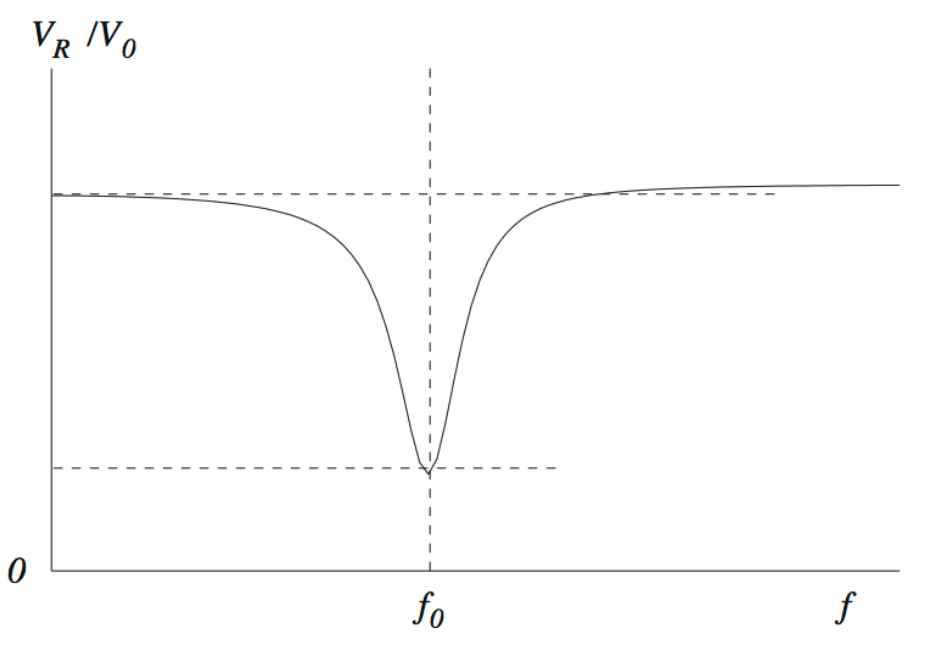
\includegraphics[width=.65\textwidth]{ParallelResonanceCurve.png}
           \caption{Parallel Resonance Curve}
           \label{fig:Parallel Resonance Curve}
        \end{center}
    \end{figure}
    We'll discuss this more in the following section.

    \subsection{The Series Resonance LRC Circuit}\label{sec:Series Resonance}
    In this set-up we have all three components, the inductor, capacitor, and resistor, in series, as 
    below.
    \begin{figure}[H]
        \centering
            \def\svgwidth{0.5\textwidth}
            \input{SeriesResonanceCircuit.pdf_tex}
            \caption{Series Resonance Circuit}
            \label{fig:Series Resonance Circuit}
    \end{figure}
    As you might imagine, the transfer function for this configuration is slightly different to 
    \autoref{eqn:Parallel Transfer Function}. In fact we will derive it now. \newline \newline
    We begin with the definition of the transfer function:
    \begin{equation*}
        H(\omega)=\frac{V_{out}}{V_{in}}
    \end{equation*}
    where $V_{in}$ is the voltage supplied by our AC source and $V_{out}$ is the voltage drop across 
    the resistor, which we know will be 
    \begin{equation*}
        V_{out}=iR
    \end{equation*}
    but as this is a series circuit we know that the current in all the components will always be the 
    same value
    \begin{equation*}
        i=\frac{V_{in}}{|Z(\omega)|}
    \end{equation*}
    where $Z(\omega)$ is the impedance of this circuit. Again this is a series circuit so the total 
    impedance is merely the sum of the impedance of the respective components.
    \begin{align*}
        Z(\omega)&=Z_L+Z_C+Z_R\\
        &=(0+jL\omega)+(0-j\frac{1}{C\omega})+(R+0j)\\
        &=R+j(L\omega-\frac{1}{C\omega})
    \end{align*}
    where we're using $j$ as the imaginary unit. Current is not complex, which is why we have $|Z|$ 
    previously. We can calculate this value
    \begin{align*}
        |Z(\omega)|&=\sqrt{Z\cdot Z*}\\
        &=\sqrt{(R+j(L\omega-\frac{1}{C\omega}))(R-j(L\omega-\frac{1}{C\omega}))}\\
        &=\sqrt{R^2+(L\omega-\frac{1}{C\omega})^2}\\
        &=\sqrt{R^2+L^2\omega^2-2\frac{L}{C}+\frac{1}{C^2\omega^2}}\\
        &=\frac{1}{C\omega}\sqrt{C^2\omega^2R^2+L^2C^2\omega^4-2LC\omega^2+1}\\
        &=\frac{1}{C\omega}\sqrt{(C\omega R)^2+(1-LC\omega^2)^2}
    \end{align*}
    Which means that we have 
    \begin{align*}
        i&=\frac{V_{in}}{\frac{1}{C\omega}\sqrt{(C\omega R)^2+(1-LC\omega^2)^2}}\\
        &=\frac{V_{in}C\omega}{\sqrt{(C\omega R)^2+(1-LC\omega^2)^2}}\\
        \implies V_{out}&=\frac{RV_{in}C\omega}{\sqrt{(C\omega R)^2+(1-LC\omega^2)^2}}\\
        \implies H(\omega)&=\frac{RV_{in}C\omega}{V_{in}\sqrt{(C\omega R)^2+(1-LC\omega^2)^2}}
    \end{align*}
    So we have our transfer function for the series resonance circuit:
    \begin{equation}
        H(\omega)=\frac{RC\omega}{\sqrt{(C\omega R)^2+(1-LC\omega^2)^2}}
        \label{eqn:Series Transfer Function}
    \end{equation}
    This equation has the same extremum as the parallel circuit, except it has a maximum at 
    $\omega_0=\frac{1}{\sqrt{LC}}$ rather than a minimum. Plotting this function we did in 
    \autoref{fig:Parallel Resonance Curve} we get 
    \begin{figure}[H]
        \begin{center}
           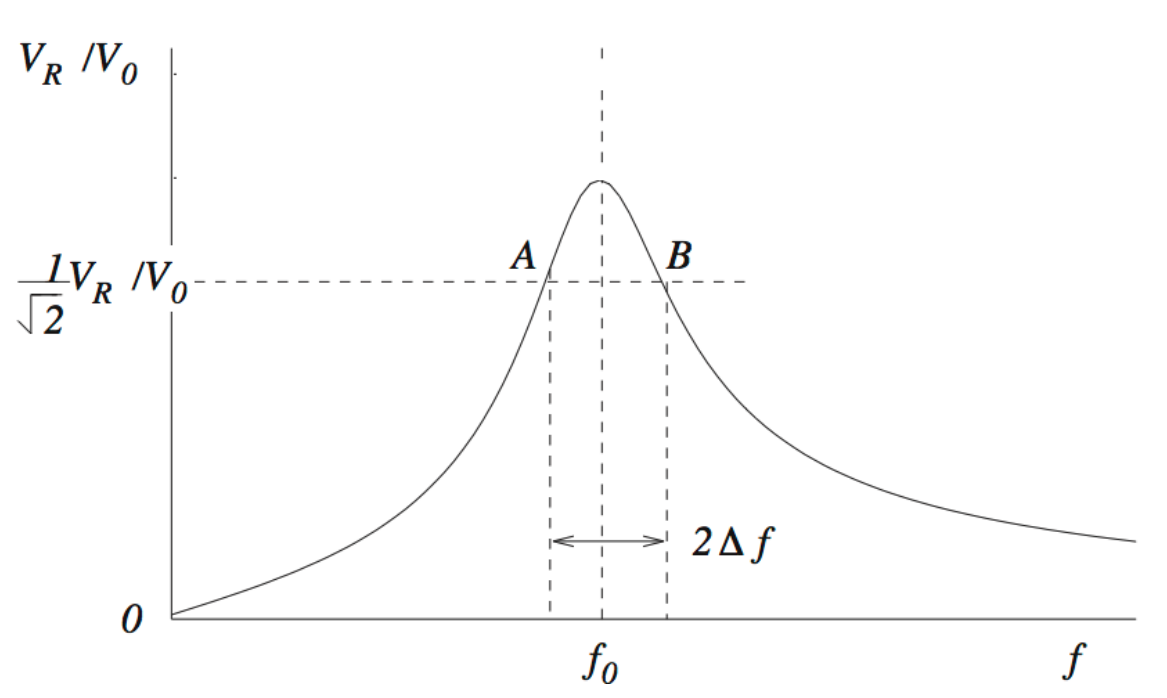
\includegraphics[width=.65\textwidth]{SeriesResonanceCurve.png}
           \caption{Series Resonance Curve}
           \label{fig:Series Resonance Curve}
        \end{center}
    \end{figure}
    These plots have $f$ along the horizontal axis as that's the input frequency but that is no problem 
    as $f=\frac{\omega}{2\pi}$. From the values of $2\Delta f$ and $f_0$ we can define a parameter 
    we call the quality factor 
    \begin{equation}
        Q=\frac{f_0}{2\Delta f}=\frac{\omega_0L}{R}
        \label{eqn:Quality Factor}
    \end{equation}
    that describes the "sharpness" of this curve, the larger $Q$ is, the sharper the curve. From 
    \autoref{eqn:Quality Factor} we see that the resistance and inductance in the circuit has an 
    impact on $Q$ and thus on the shape of the resonance curve. Note that this quality factor and its 
    associated usefulness is not unique to the series resonance circuit, it applies to the parallel 
    circuit too and we will use this in later sections to analyse specific circuits.

    \section{Experiment}\label{sec:Experiment}
    In the experimental section of this report we will be investigating the behaviour of both the 
    parallel and series resonance circuits by way of setting them up on a breadboard to see how they 
    behave in reality, as well as using a simulation of each. 
    \subsection{Apparatus}\label{sec:Apparatus}
    We used the following items, all with standard measurement uncertainty of 2\%:
    \begin{itemize}
        \item 1 1 k$\Omega$ resistor (actual measured value 984.4 $\Omega$).
        \item 2 100 $\Omega$ resistors (actual measured value 98.0 and 98.6 $\Omega$).
        \item 1 96.51 nF capacitor (actual measured value 93.94 nF).
        \item 1 70 mH inductor (actual measured value 73.62 mH).
        \item 1 myDAQ.
        \item 1 screwdriver.
        \item 1 function generator.
        \item 1 digital oscilloscope.
        \item 1 breadboard.
        \item Wire (with negligible resistance).
    \end{itemize}
    Our parallel circuit was set up with the 1 k$\Omega$ resistor and the series circuit was set up 
    with the two 100 $\Omega$ resistors in series to achieve a total resistance of 200 $\Omega$. 
    They were set up in the same configuration as in \autoref{fig:Parallel Resonance Circuit} and 
    \autoref{fig:Series Resonance Circuit}. 

    \subsection{Method and Results}\label{sec:Method and Results}
    To collect our data (thanks Prof Blumenthal) we started off using the function generator to apply 
    a sinusoidal alternating voltage of 1 Volt peak-to-peak across the parallel and series circuits 
    with the oscilloscope 
    measuring the voltage across the resistor. By adjusting the frequency of the function generator 
    we were able to find the point at which the voltage across the resistor was minimised or maximised, 
    depending on the type of circuit. The oscilloscope displays for each circuit are pictured 
    in \autoref{fig:Parallel Resonance Scope} and \autoref{fig:Series Resonance Scope}
    \begin{figure}[h]
        \begin{center}
           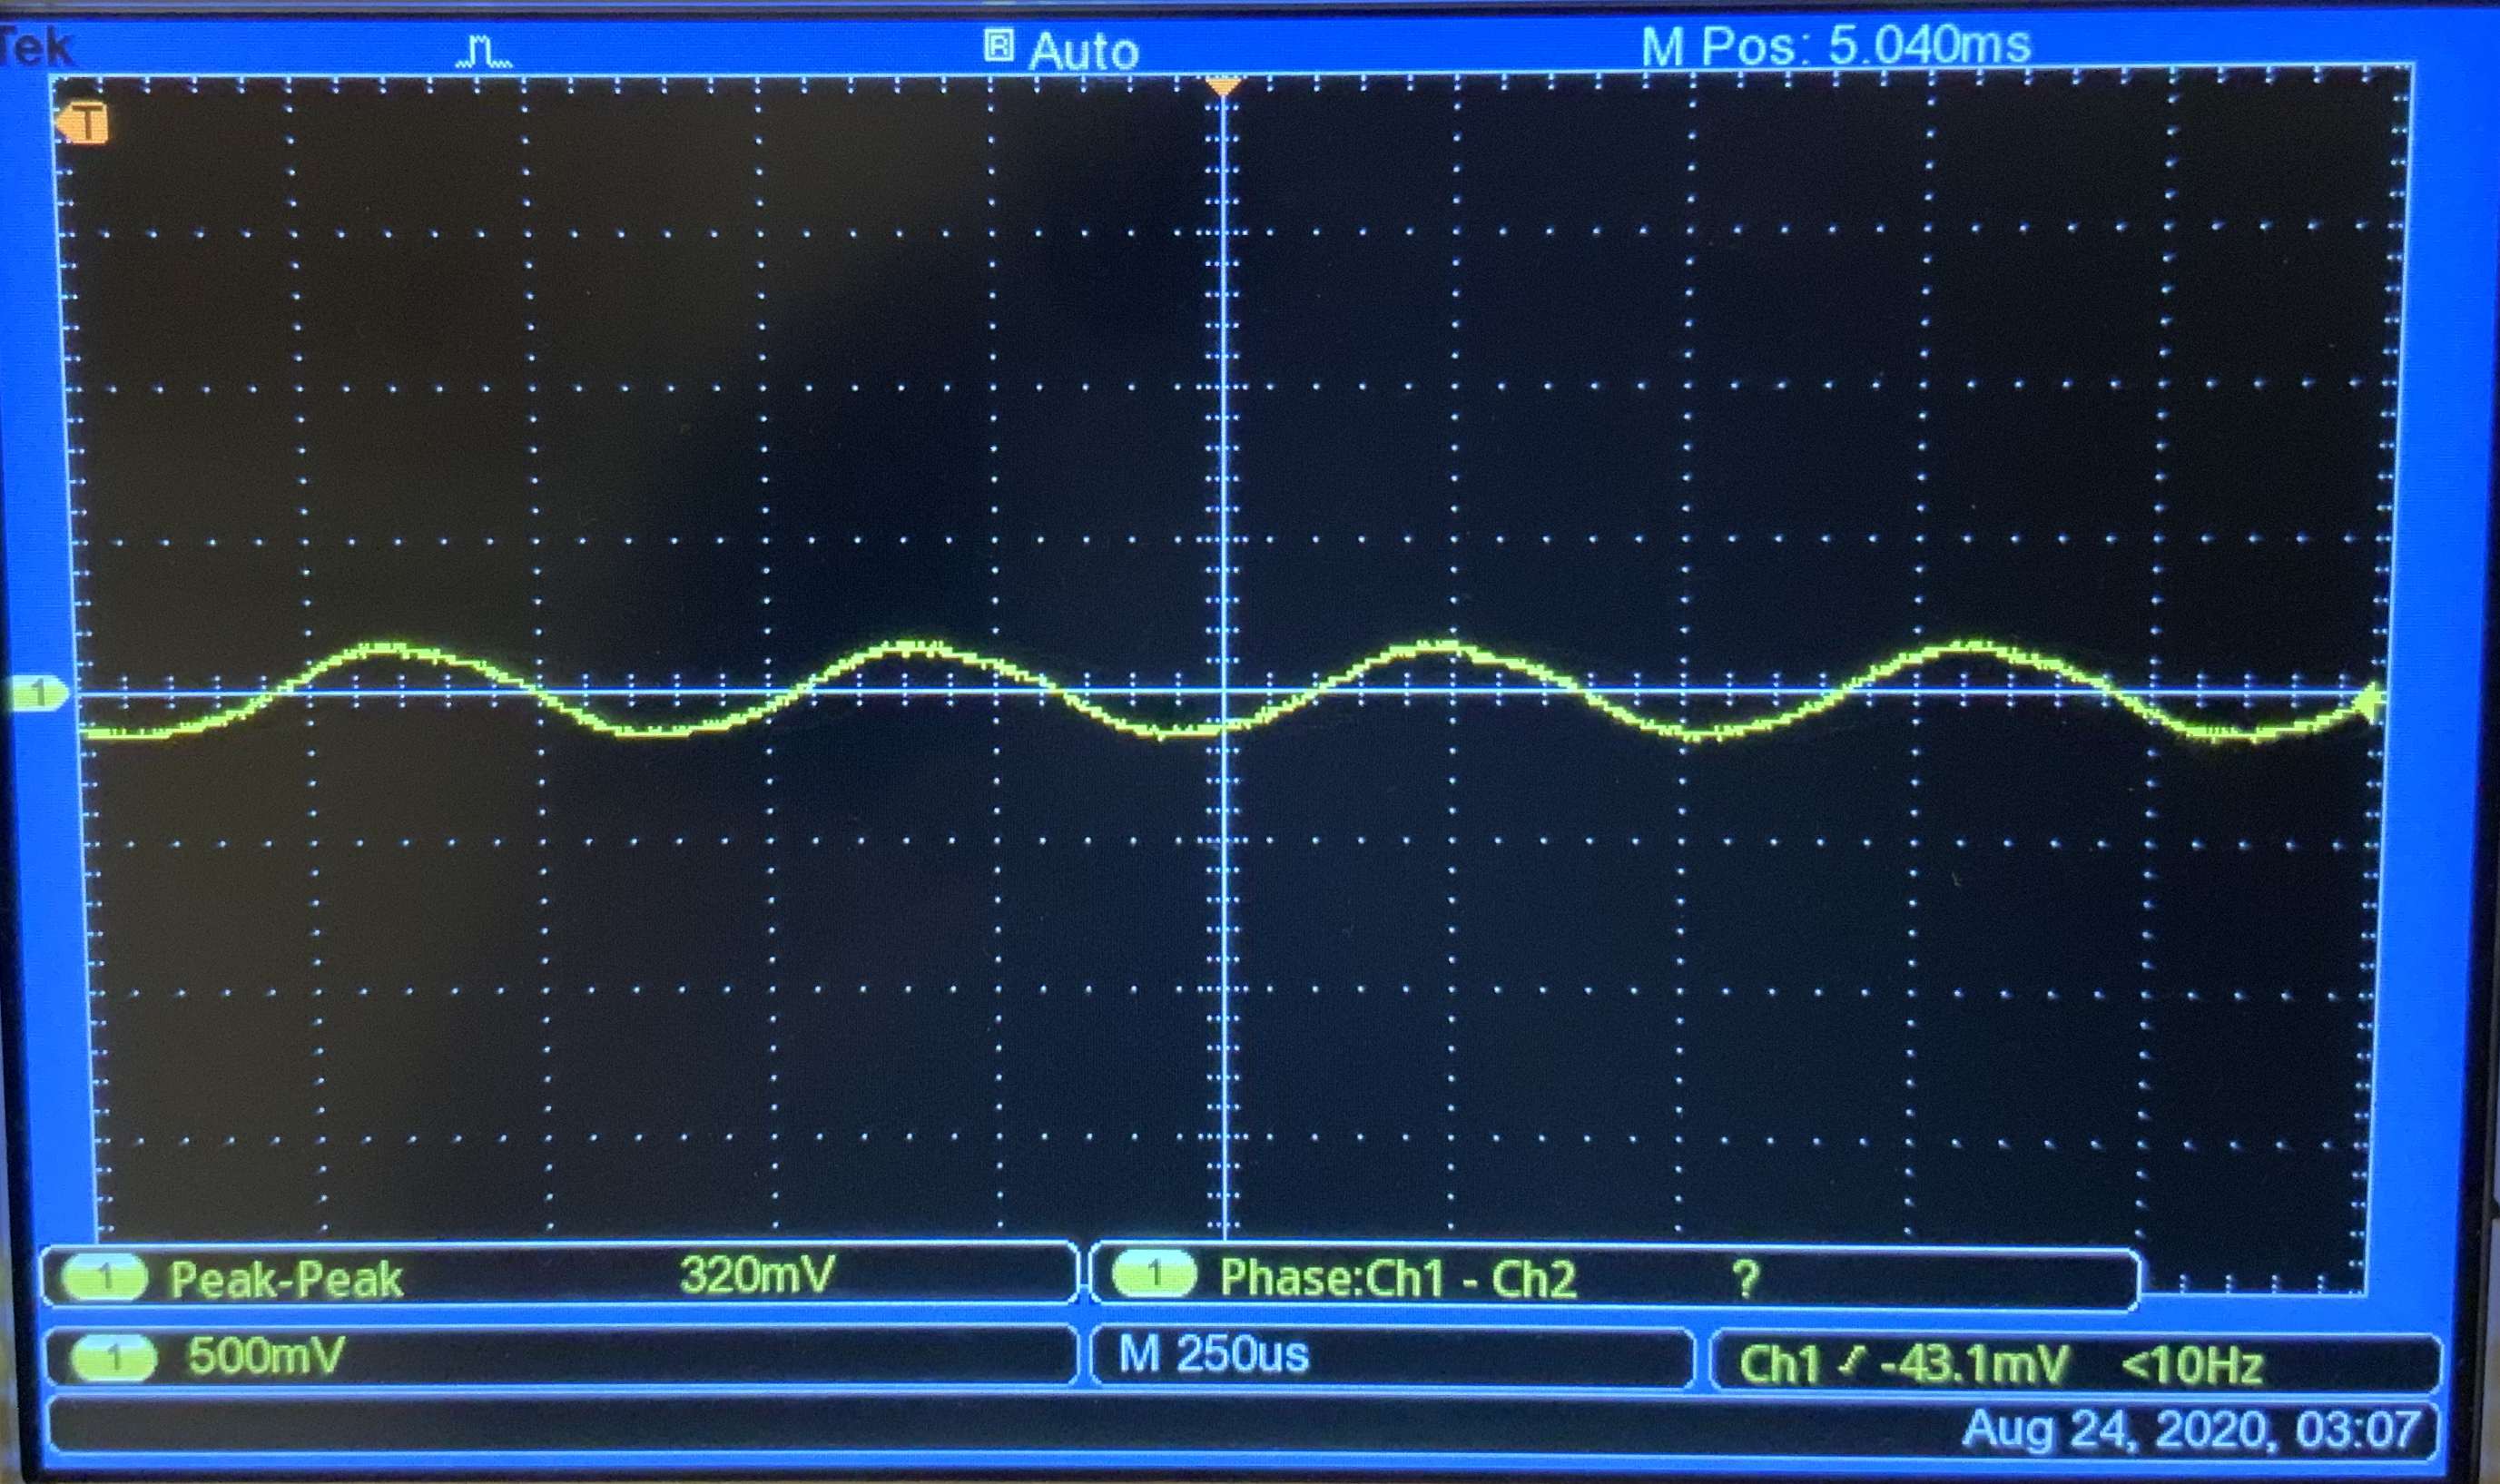
\includegraphics[width=.65\textwidth]{Parallel_Resonance_Scope.jpg}
           \caption{Parallel Resonance Circuit at resonance}
           \label{fig:Parallel Resonance Scope}
        \end{center}
    \end{figure}
    \begin{figure}[h]
        \begin{center}
           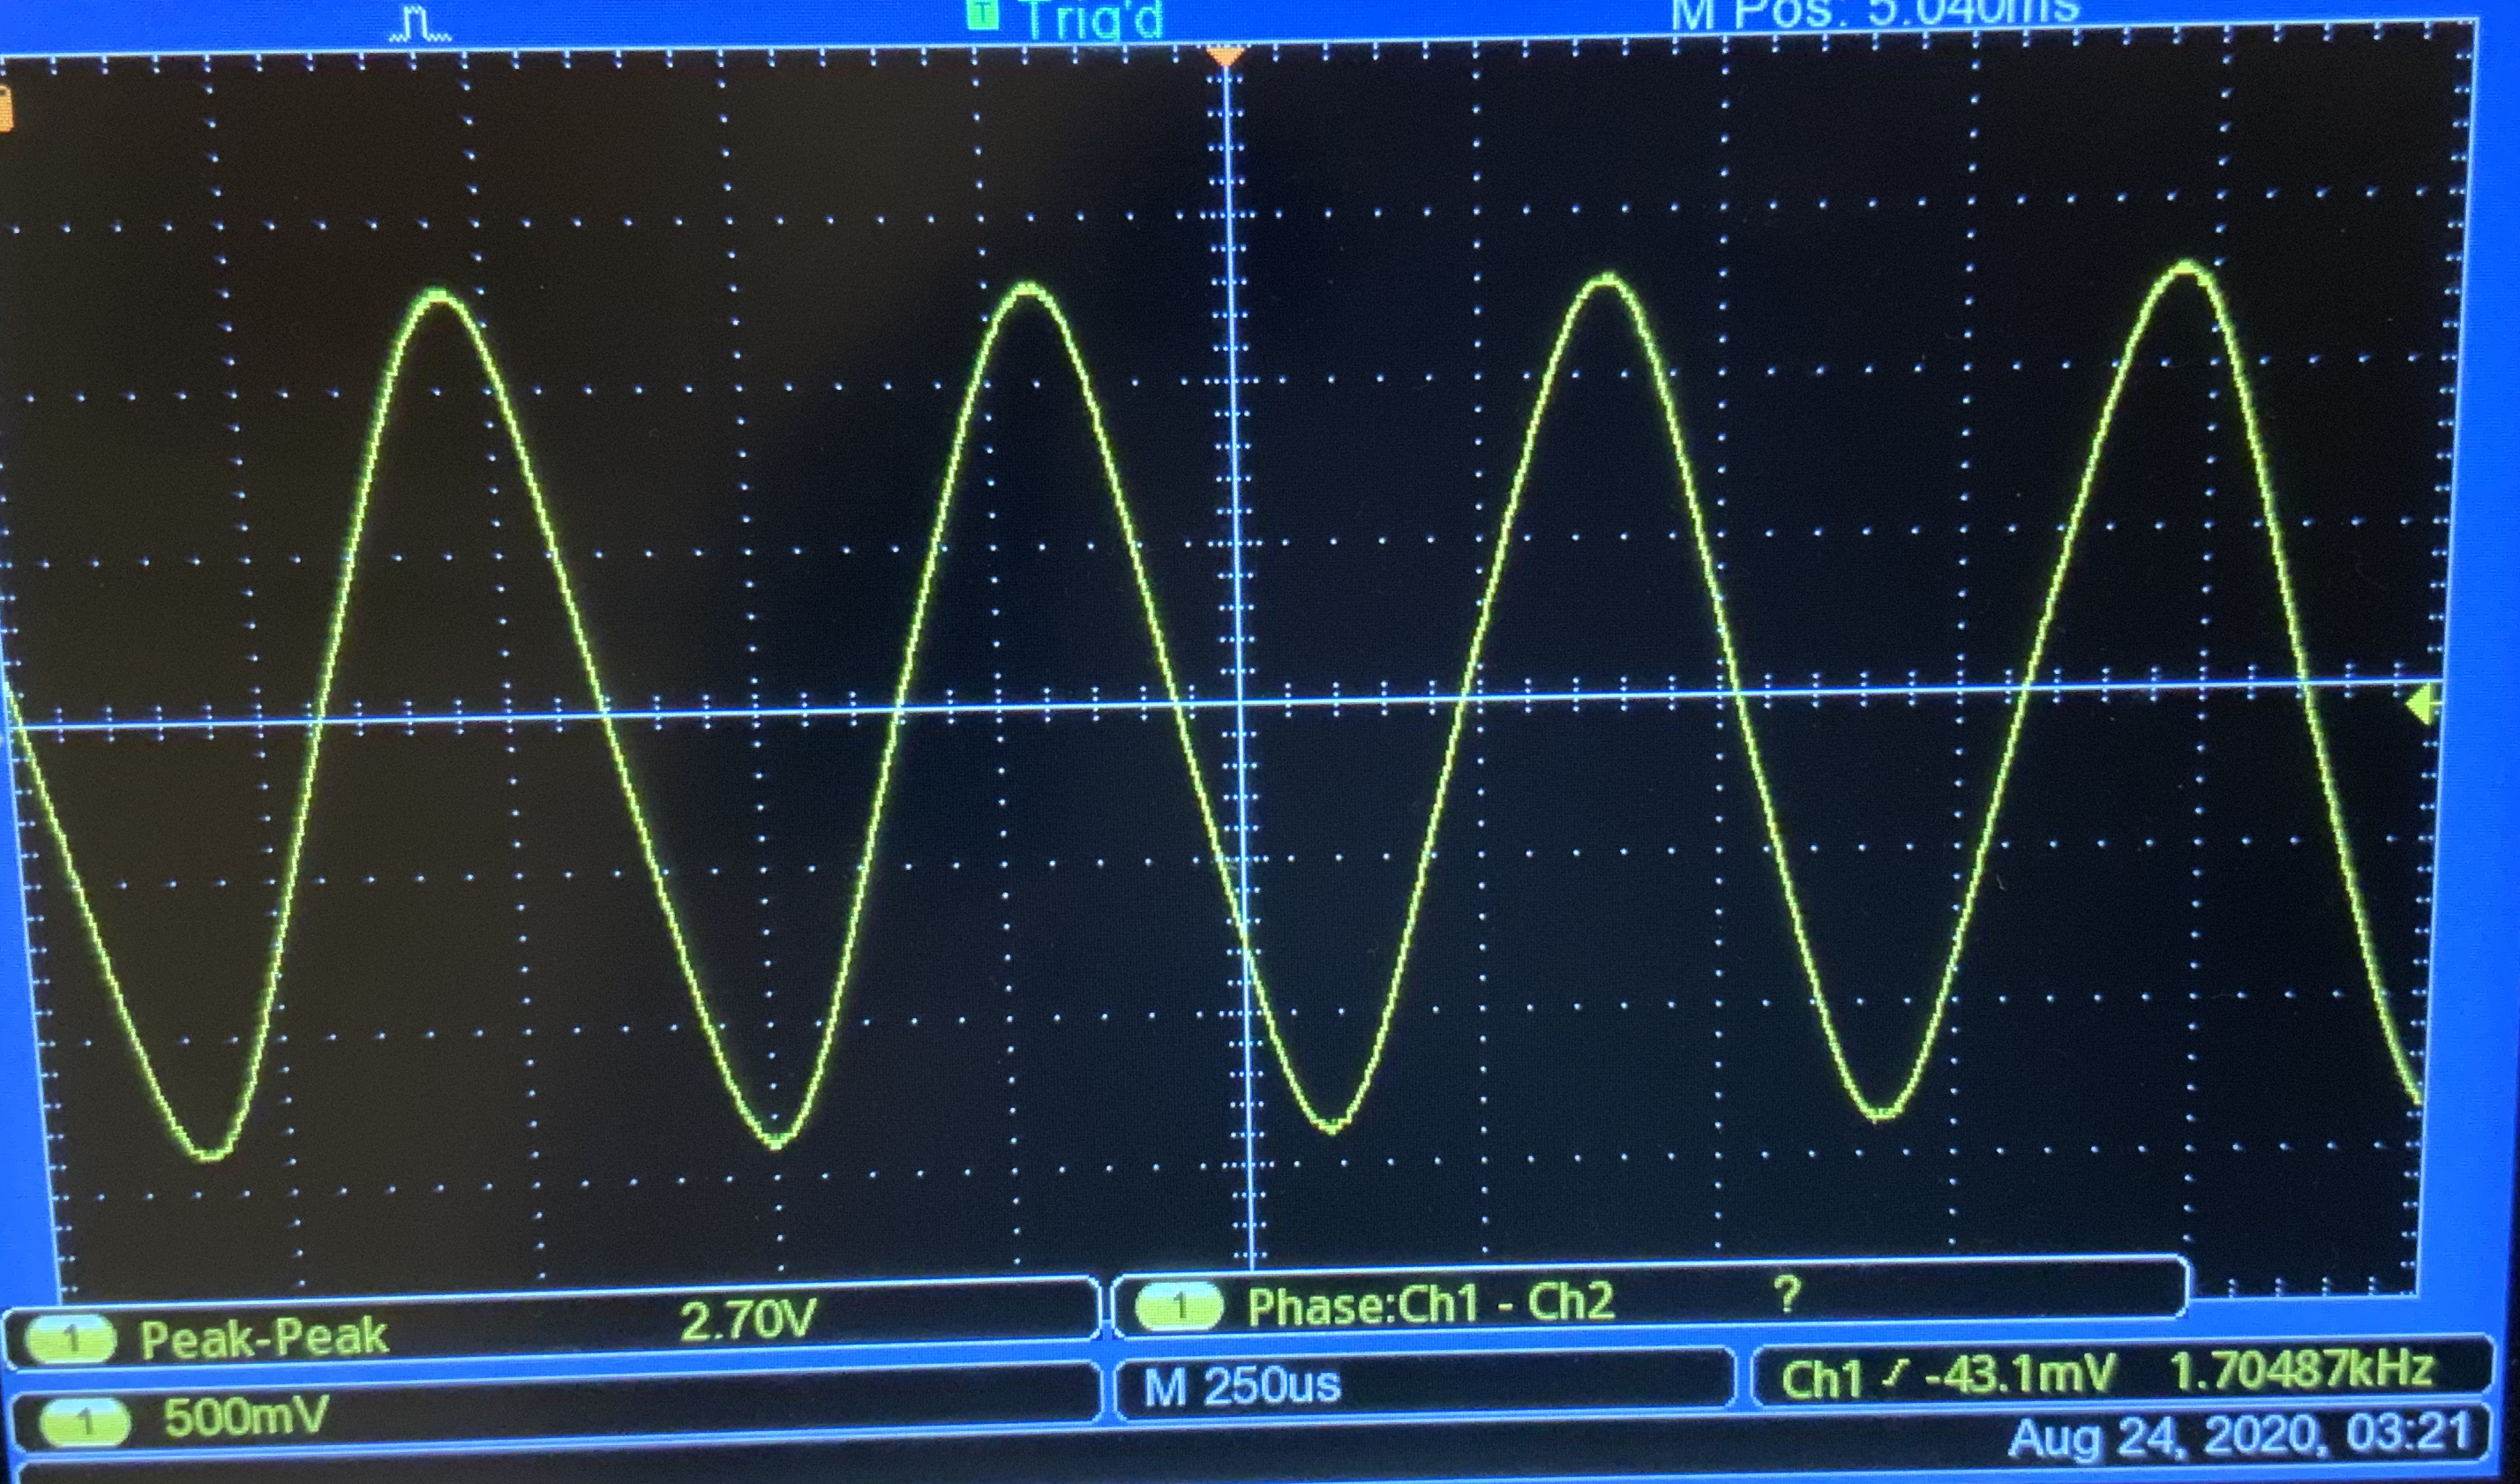
\includegraphics[width=.65\textwidth]{Series_Resonance_Scope.jpg}
           \caption{Series Resonance Circuit at resonance}
           \label{fig:Series Resonance Scope}
        \end{center}
    \end{figure}
    \newline
    \newline
    Starting with \autoref{fig:Parallel Resonance Scope}, we counted one wavelength to be 11 small 
    divisions, with one division on either side as the bounds of the pdf. One division is 
    $\SI{0.5e-4}{\second}$ and this is an analogue reading, so our uncertainty is 
    $u=\frac{a}{2\sqrt{6}}$. That gives us a wavelength of $\lambda=\SI{5.5\pm0.2641e-4}{\second}$. 
    As we know, $f=\frac{1}{\lambda}$, and the uncertainty is given by 
    $u(f)=\frac{u(\lambda)}{\lambda^2}$, which was derived from the multiplicative propagation 
    equation. This gives us a resonant frequency of $f_0=1818.18\pm67.48\;\si{\hertz}$. \newline
    \newline
    For the series circuit, \autoref{fig:Series Resonance Scope}, we counted 12 small divisions 
    with the same upper and lower bound. Doing the same calculations and uncertainty propagations 
    we found the resonant frequency to be $f_0=1666.67\pm73.37\;\si{\hertz}$. The expected value for 
    both circuits can be found from $\omega_0=2\pi f_0=\frac{1}{\sqrt{LC}}$. If we use the measured 
    values for $L$ and $C$ with uncertainties of 2\% we get $f_0=1913.802\pm27.064\;\si{\hertz}$, 
    where the uncertainty is given by
    \begin{equation*}
        u(f)=\sqrt{\frac{L^2u(C)^2+C^2u(L)^2}{4C^3L^3}}
    \end{equation*} 

    Next we used the \texttt{LCsim.exe} program to simulate the parallel and series circuits with 
    a range of different resistance values to investigate how the value of R affects the value of $Q$. 
    We simulated two circuits with the same inductance and capacitance values as the real circuits we 
    used (70 mH and 96.51 nF) and ran each circuit separately with 100, 200, 400, and 1000 $\Omega$s 
    of resistance, 1 Volt peak-to-peak, and from 1000 to 4000 Hz with 2000 data points. The program 
    can export as text so we copied the outputs into \text{.txt} files and did our usual plotting 
    procedure. We then used \texttt{scipy.optimize.curve\_fit} to fit the data to the relevant 
    transfer function. The results are in \autoref{fig:Parallel Resonance Circuit} and 
    \autoref{fig:Series Resonance Circuit}.
    \begin{figure}[H]%
        \centering
        \subfloat[100 Hz]{\scalebox{0.4}{\subimport{Plots}{Parallel_Freq_Sweep_100.pgf}}}
        \,
        \subfloat[200 Hz]{\scalebox{0.4}{\subimport{Plots}{Parallel_Freq_Sweep_200.pgf}}}
        \,
        \subfloat[400 Hz]{\scalebox{0.4}{\subimport{Plots}{Parallel_Freq_Sweep_400.pgf}}}
        \,
        \subfloat[1000 Hz]{\scalebox{0.4}{\subimport{Plots}{Parallel_Freq_Sweep_1000.pgf}}}
        \caption{Parallel Circuit Simulation}
        \label{fig:Parallel Simulation}
    \end{figure}
    \begin{figure}[H]%
        \centering
        \subfloat[100 Hz]{\scalebox{0.4}{\subimport{Plots}{Series_Freq_Sweep_100.pgf}}}
        \,
        \subfloat[200 Hz]{\scalebox{0.4}{\subimport{Plots}{Series_Freq_Sweep_200.pgf}}}
        \,
        \subfloat[400 Hz]{\scalebox{0.4}{\subimport{Plots}{Series_Freq_Sweep_400.pgf}}}
        \,
        \subfloat[1000 Hz]{\scalebox{0.4}{\subimport{Plots}{Series_Freq_Sweep_1000.pgf}}}
        \caption{Series Circuit Simulation}
        \label{fig:Series Simulation}
    \end{figure}
    We'd like to mention here that the \texttt{LCsim.exe} program seems to have a maximum resolution 
    of 0.01 Volts, which is the reason that the data above looks choppy. Despite this it seems that 
    the \texttt{curve\_fit} function can still approximate the function well because the steps seem 
    to even each other out. \newline \newline
    And finally, in order to investigate the transfer function for these two circuits, we used the 
    myDAQ to apply a range of frequencies of alternating voltage with 1 Volt peak-to-peak to the 
    circuits described in \autoref{sec:Apparatus}. The myDAQ also recorded the voltage across the 
    resistor. We could then plot that data and use \texttt{curve\_fit} to fit it to the relevant 
    transfer function. The results are in \autoref{fig:Parallel Frequency Sweep}, 
    \autoref{fig:Series Frequency Sweep}, and \autoref{tbl:Resonant Frequency and Quality Factor}.
    The $Q$ values were calculated from \autoref{eqn:Quality Factor}.

    \begin{figure}[H]
        \begin{center}
           \scalebox{.7}{\subimport{Plots}{Parallel_Freq_Sweep.pgf}}
           \caption{Parallel Frequency Sweep}
           \label{fig:Parallel Frequency Sweep}
        \end{center}
    \end{figure}
    \begin{figure}[H]
        \begin{center}
           \scalebox{.7}{\subimport*{Plots}{Series_Freq_Sweep.pgf}}
           \caption{Series Frequency Sweep}
           \label{fig:Series Frequency Sweep}
        \end{center}
    \end{figure}

    \begin{table}[H]
        \begin{minipage}{0.5\textwidth}
            \centering
            \textbf{Parallel} \\
            \begin{tabular}{c c}
                \hline
                $f_0$: & $1926.80\pm38.54\; \si{\hertz}$\\
                $L$: & $\SI{65.78\pm3.33e-3}{\henry}$\\
                $R$: & $931.98\pm49.22\;\si{\ohm}$\\
                $C$: & $\SI{106.41\pm5.41e-09}{\farad}$\\
                Scale Factor: & $0.48716\pm0.00059$\\
                $Q$: & $1.17\pm0.082$
            \end{tabular}
        \end{minipage}
        \vline\;
        \begin{minipage}{0.5\textwidth}
            \centering
            \textbf{Series} \\
            \begin{tabular}{c c}
                \hline
                $f_0$: & $1866.90\pm37.34\; \si{\hertz}$\\
                $L$: & $\SI{73.31\pm3.25e-3}{\henry}$\\
                $R$: & $272.95\pm12.66\;\si{\ohm}$\\
                $C$: & $\SI{98.954\pm4.097e-09}{\farad}$\\
                Scale Factor: & $ 0.3888\pm0.0014$\\
                $Q$: & $3.15\pm0.18$
            \end{tabular}
        \end{minipage}
        \caption{Resonant Frequency and Quality Factor for Parallel and Series Resonant Circuits}
        \label{tbl:Resonant Frequency and Quality Factor}
    \end{table}
    On the uncertainties for these values, we used the 2\% accuracy rating for the equipment used 
    in order to get the uncertainty of $f_0$, the resonant frequency. The uncertainties of $L$, $R$, 
    $C$, and the Scale Factor we used Monte Carlo methods, particularly the Jackknife method to 
    estimate the uncertainties as these values came from the optimal fitting parameters that 
    \texttt{curve\_fit} gave us. $Q$ was determined from \autoref{eqn:Quality Factor} and the 
    uncertainty was determined from propagating the Jackknife uncertainties through that equation 
    using the multiplicative propagation equation:
    \begin{equation*}
        z=xy \implies u(z)=|xy|\sqrt{\left(\frac{u(x)}{x}\right)^2+\left(\frac{u(y)}{y}\right)^2}
    \end{equation*}
    All of the code that did this analysis is in \autoref{app:Parallel Freq Sweep} and 
    \autoref{app:Series Freq Sweep}, being modified slightly to loop through different files.

    \section{Discussion and Recommendations}\label{sec:Discussion and Recommendations}
    \subsection{Resonance Frequency Search}\label{sec:Resonance Frequency Search}
    The two resonant frequencies found in \autoref{sec:Method and Results} from examining 
    \autoref{fig:Parallel Resonance Scope} and \autoref{fig:Series Resonance Scope} were 
    \begin{align*}
        \text{Parallel:}&\hspace{25pt}f_0=1818.18\pm67.48\;\si{\hertz}\\
        \text{Series:}&\hspace{25pt}f_0=1666.67\pm73.37\;\si{\hertz}\\
        \text{Expected:}&\hspace{25pt}f_0=1913.802\pm27.064\;\si{\hertz}
    \end{align*}
    These values do not agree. The reason for this discrepancy is likely due to the lack of control 
    we have when finding the resonant frequency as the effective resolution on the oscilloscope when 
    modulating the driving frequency is quite low, so it's hard to find the exact resonant frequency. 
    To improve this experiment we recommend using the methods we used when analysing the myDAQ data as 
    it's much more definite than just guessing while looking at an oscilloscope. 

    \subsection{Circuit Simulation}\label{sec:Circuit Simulation}
    To investigate the relationship between resistance and the quality factor, we look at 
    \autoref{fig:Parallel Frequency Sweep} and \autoref{fig:Series Frequency Sweep}. Looking at the 
    parallel circuit first, the function clearly becomes more sharp the higher the resistance is, so 
    $Q\propto R$ for the parallel resonance circuit. The opposite is true for series; as the resistance 
    increases the function becomes less sharp, so we have $Q\propto \frac{1}{R}$ for the series 
    resonance circuit. To improve this part of the experiment we might want to use more simulations 
    and find the relationship between $Q$ and $R$ quantitatively. 

    \subsection{Frequency Sweep}\label{sec:Frequency Sweep}
    Finally we will analyse the results we found in 


    \newpage
    \section{Appendix}
    \setcounter{figure}{0} \renewcommand{\thefigure}{A.\arabic{figure}}
    \lstinputlisting[caption=Parallel Frequency Sweep, label=app:Parallel Freq Sweep, style=appendix]{Parallel_Freq_Sweep.py}
    \lstinputlisting[caption=Series Frequency Sweep,label=app:Series Freq Sweep, style=appendix]{Series_Freq_Sweep.py}
    


    
\end{document}